\documentclass[11pt,a4paper,oneside]{article}
    \usepackage{a4wide}
    \usepackage{epsfig}
    \usepackage{amsmath}
    \usepackage{tabu}
    \usepackage{amsfonts}
    \usepackage{latexsym}
    \usepackage[utf8]{inputenc}
    \usepackage{listings}
    \usepackage{color}
    \usepackage{titlesec}    
    \usepackage{enumitem}
    \usepackage[catalan]{babel}
    \usepackage{newunicodechar}
    \usepackage{graphicx}
    \usepackage{subcaption}
    \usepackage{float}
    \usepackage{xcolor}
    \usepackage{pgf, tikz}
    \usepackage{listings}
    \usepackage{eurosym}
    \usepackage[figuresleft]{rotating}
    \usepackage{mathtools}
    \usepackage{pdfpages}
  \setcounter{tocdepth}{2}
  \setcounter{secnumdepth}{4}
  
  \newunicodechar{Ŀ}{\L.}
  \newunicodechar{ŀ}{\l.}
  \definecolor{dkgreen}{rgb}{0,0.6,0} 
  \definecolor{gray}{rgb}{0.5,0.5,0.5}
  \definecolor{mauve}{rgb}{0.58,0,0.82}
  
  
\definecolor{maroon}{rgb}{0.5,0,0}
\definecolor{darkgreen}{rgb}{0,0.5,0}
\lstdefinelanguage{XML}
{
  basicstyle=\ttfamily,
  morestring=[s]{"}{"},
  morecomment=[s]{?}{?},
  morecomment=[s]{!--}{--},
  commentstyle=\color{darkgreen},
  moredelim=[s][\color{black}]{>}{<},
  moredelim=[s][\color{red}]{\ }{=},
  stringstyle=\color{blue},
  identifierstyle=\color{maroon}
}

  \usepackage{hyperref}
  \hypersetup{
    colorlinks=false, %set true if you want colored links
    linktoc=all,     %set to all if you want both sections and subsections linked
    linkcolor=blue,  %choose some color if you want links to stand out
  }
  
  \setlength{\footskip}{50pt}
  \setlength{\parindent}{0cm} \setlength{\oddsidemargin}{-0.5cm} \setlength{\evensidemargin}{-0.5cm}
  \setlength{\textwidth}{17cm} \setlength{\textheight}{23cm} \setlength{\topmargin}{-1.5cm} \addtolength{\parskip}{2ex}
  \setlength{\headsep}{1.5cm}
  
  \renewcommand{\contentsname}{Continguts}
  % \titleformat{\chapter}[display]
  % {\normalfont\bfseries}{}{0pt}{\Large}
  \titleformat{\chapter}[block]
  {\normalfont\LARGE\bfseries}{\thechapter.}{1em}{\LARGE}
  \titleformat{\section}[block]
  {\normalfont\Large\bfseries}{\thesection.}{1em}{\Large}
  
  \begin{document}
  % \title{(title)}
  % \author{(author)}
  % \maketitle
  \begin{titlepage}
    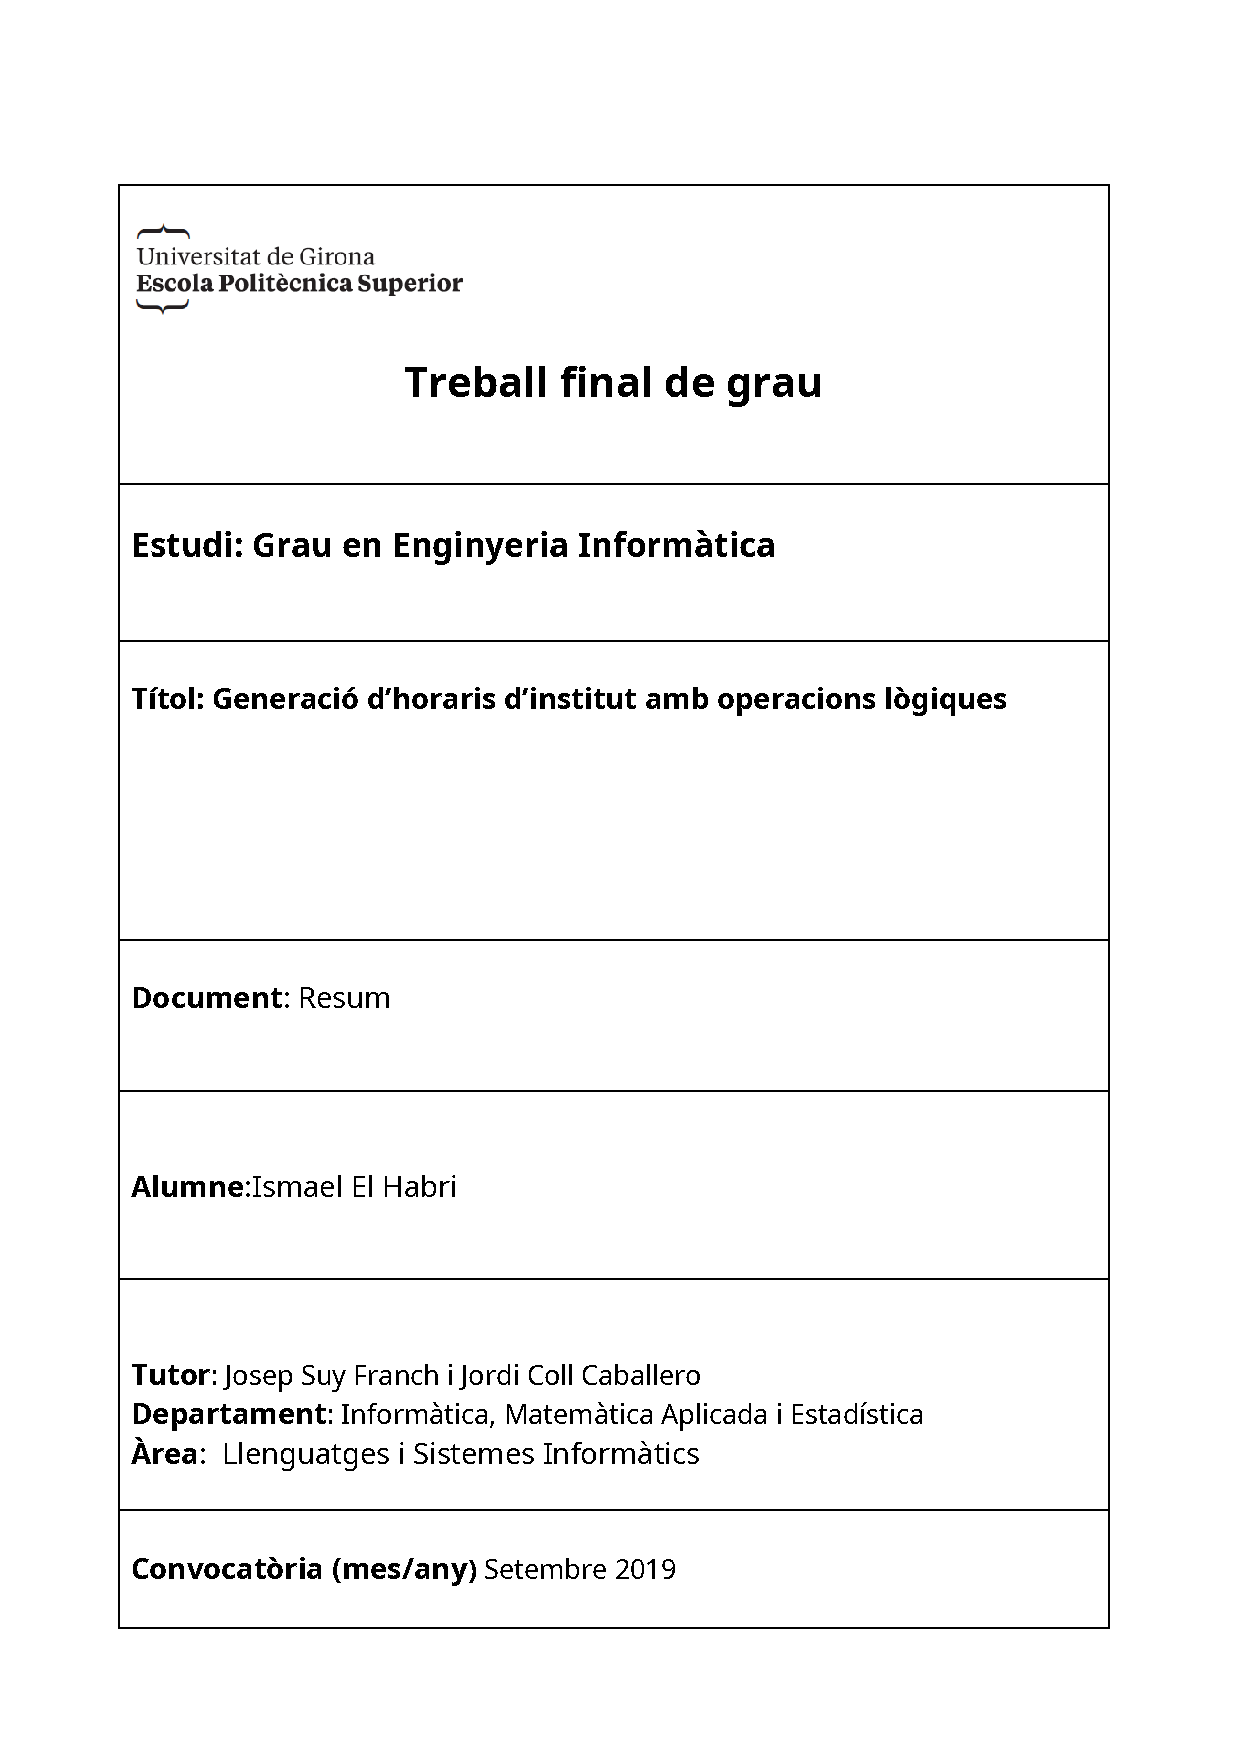
\includepdf[pages=1]{portada_resum.pdf}
  \end{titlepage}

  
  \tableofcontents \newpage

  \section{Introducció}
  
  La confecció d'horaris és un problema recurrent amb el qual es troben els instituts que amaga una alta combinatòria, 
  dificultant-ne molt la seva elaboració manual donat que s'han de prendre moltíssimes decisions a cegues,
  fa que sigui molt probable cometre errors en la confecció.

  El HSTT (High School TimeTabling) consisteix en la solució de forma automàtica d'aquest problema d'alta complexitat (NP). 
  Així doncs, el que s'intenta és la configuració automàtica d'horaris d'institut partint d'una sèrie de recursos 
  (per exemple: aules, professors, assignatures, grups) i repartir-los de manera que sigui viable i tenint en compte 
  de manera total o parcial les preferències del professorat respecte a horaris, continuïtat, grups, etc. 
  Tot això, fa que el problema sigui molt difícil de resoldre a causa del gran nombre de combinacions possibles entre els diferents recursos.
  
  Afegint dificultat al problema, depenguen del país del qual estiguem parlant existeixen una gran diversitat de requisits propis, degut a les característiques pròpies del sistema d'estudis secundaris de cada lloc.



  \subsection{Objectius}
  Els objectius d'aquest treball són els següents:
  \begin{itemize}
    \item Aprofundir sobre el problema de la generació d'horaris en sí i sobre els problemes de satisfacció de restriccions en general i les tècniques que s'utilitzen per resoldre'ls, com ara, SAT i les seves diverses extensions.
    \item Desenvolupar un generador d'horaris automàtic utilitzant les tècniques estudiades anteriorment. 
    Aprofitant les eines relacionades que s'han desenvolupat recentment pel grup de recerca Lògica i Programació, 
    s'intentarà resoldre el problema en un temps raonable i intentar trobar la millor solució possible. 
    Això que es preveu molt complicada d'aconseguir en un temps raonable en les instàncies grosses.
    
  \end{itemize}
  
  \subsection{Estudi de viabilitat}
  Per tal de realitzar aquest projecte farà falta el software necessari per poder tractar un fitxer XML, codificar una instància del problema en C++ i resoldre-la amb un \textit{solver} SAT o d'alguna extensió de SAT. 
  Abans d'iniciar el projecte, s'ha comprovat l'existència d'aquest software i que aquest estigués disponible de forma gratuïta, de fet, tot el software que s'utilitzi en aquest projecte serà de codi obert.

  Per part dels requisits de maquinari, tot i que HSTT és un problema dur, 
  després de veure el treball previ realitzat en aquest mateix problema i d'altres de característiques semblants, s'ha determinat que la meva màquina d'ús diari és més que suficient per a tal de realitzar el desenvolupament del generador d'horaris.

  Pel que fa a l'habilitat de desenvolupar aquest treball s'ha determinat que era possible gràcies al fet que
  el grup de recerca Lògica i Programació ha treballat i aconseguit solucionar problemes semblants de forma exitosa utilitzant tècniques innovadores. 
  Utilitzant els avenços fets pel grup s'ha decidit que es podria desenvolupar el treball en el marc de temps desitjat.

  \subsection{Metodologia}

  El model de desenvolupament que s'ha triat en aquest treball ha estat el model de prototips (o prototipatge), 
  que consisteix a crear, com el nom indica, prototips del programari que es pretén crear, és a dir, versions incompletes del software que s'està desenvolupant.
  Generalment, un prototip només compleix alguns dels requeriments del sistema i pot no tenir res a veure amb el producte final.
  
  \section{Marc de Treball}
   Aquest treball s'emmarca dins del grup de recerca de Lògica i Programació (LiP) del departament d'Informàtica, Matemàtica Aplicada i Estadística (IMAE) de la Universitat de Girona. 
    En el treball s'utilitzaran les eines desenvolupades recentment en el grup de recerca, per ser exactes, la API SMT feta en C++ pel Dr. Jordi Coll. 
    Aquesta API permet codificar problemes SAT, MaxSAT i SMT per a diferents \textit{solvers} de forma transparent a aquest i té implementades les diferents restriccions de cardinalitat i pseudo-booleanes en les diferents possibles codificacions. 
    També inclou diferents algoritmes d'optimització implementats.

    La resta del treball previ seria el treball final de grau fet el 2015 per en Cristòfor Nogueira, el qual també consisteix en la confecció d'horaris d'institut.

  \section{Implementació}


  El model està pensat per treballar a centrant-nos en els Events (o assignatures), 
  els quals podríem definir com una reunió a la que es presenten diferents recursos 
  i la nostra feina és la de decidir en quins espais de temps dels disponibles fiquem cada reunió d'aquestes.

  Les variables del model són les següents:
  \begin{itemize}
    \item $Xt_{0,0} . . . Xt_{|Events|-1,|Times|-1}$\\Per cada event tenim tantes variables com espais de 
    temps tingui la instància.
    \item $Xs_{0,0} . . . Xs_{|Events|-1,|Times|-1}$\\Per cada event tenim tantes variables com espais de temps tingui la instància.
    \item $Xd_{0,1,0} . . . Xd_{|Events|-1, event.duration, |Times|-1}$\\ Per cada event i cada possible duració d'aquest tenim una variable. 
  \end{itemize}

  Per poder dotar les variables del model de semàntica caldrà afegir certes clàusules, que en direm clàusules de \textit{channeling}. A continuació s'enumeren:
  \begin{itemize}
    \item Si un event comença a una hora determinada, llavors té una duració: \begin{center} $\forall e \in 0 ... |Events|-1$ $\forall i \in 0 ... |Times|-1$ \\$exactily\_one(\neg Xs_{e,i} \vee \{ \forall j \in 1 ... e.duration$ $Xd_{e,j,i}\})$\end{center}
    \item Si un event té lloc a t però no a t-1, és que comença: \begin{center} $\forall e \in 0 ... |Events|-1$ $\forall i \in 0 ... |Times|-1$ \\$\neg Xt_{e,i} \vee Xt_{i-1} \vee Xs_i$ \end{center}
    \item Si un event comença amb duració d, llavors té lloc en d hores consecutives: \begin{center} 
      $\forall e \in 0 ... |Events|-1$ $\forall d in 1 ... e.duration$ $\forall i \in 0 ... |Times|-1$ $\forall j \in i ... i+d-1$ \\
      $\neg Xd_{e,d,i} \vee Xt_{e,j}$
    
    \end{center}
  \end{itemize}

  A partir d'aquí s'han implementat les diferents clàusules necessaries per a codificar les múltiples restriccions suportades.


  \section{Resultats}

  Per avaluar els resultats obtinguts s'han comparat 
  els temps obtinguts i les variables i clàusules generades pel generador d'horaris desenvolupat utilitzant
  diferents combinacions de codificacions de les restriccions de cardinalitat 
  i les restriccions \textit{at\_most\_one}.
  
  Els resultats de resolució obtinguts han semblat positius. 
  Els temps d'execució per determinar si una instància és satisfactible i donar un horari viable per ella, han estat molt bons. 
  Cal tenir en compte que algunes de les instàncies provades son reals, i s'han arribat a resoldre instàncies de fins a prop de 40 milions de clàusules.
  Per això crec que es pot determinar que l'habilitat d'oferir un horari viable per a qualsevol instància de les treballades és molt positiva.

  Per altra banda, l'habilitat de buscar la millor solució en un temps raonable 
  no es pot determinar com a bona. A part de la primera instància, 
  la qual es resol molt ràpidament, el generador no és capaç d'obtenir la solució optima.
   A més, comparant el cost de la solució trobada amb les dues altres solucions de la instància, l'obtinguda pel generador desenvolupat en aquest treball resulta ser molt més elevat.

  \section{Conclusions}

  Durant el desenvolupament d'aquest treball s'han estudiat, repassat i aplicat diverses tècniques de programació per restriccions, 
  sobretot les diferents codificacions de restriccions globals a CNF per SAT i SMT, que s'han acabat utilitzant en el generador d'horaris que s'ha creat. 

  Pel que fa el generador desenvolupat al llarg d'aquest treball, tot i estar molt lluny de la perfecció, 
  ha permès posar a prova les diferents codificacions de les restriccions globals vistes en el treball 
  i compleix amb els objectius marcats al principi del treball. El generador és capaç de resoldre el problema en un temps raonable (la instància que tarda més és la 4, que ens tarda menys de 10 minuts), 
  excepte la instància 7, la qual a l'intentar resoldre, ens quedem sense memòria. Cal tenir en compte però que les instàncies 4 i 6 són problemes de instituts reals de Brazil, i els temps d'execució resultants en aquestes instàncies són molt positius.
  Per altra part, la cerca de la solució òptima, ha resultat bastant negativa, tot i tenir bons temps amb l'optimitzador dicotòmic en la instància més petita, generalment ha resultat impossible aconseguir bons resultats. 
  A més, comparant l'optimalitat de la solució obtinguda amb les altres solucions existents de la instància, aquestes últimes han resultat ser molt superiors a les obtingudes en aquest treball.


  Pel que fa el treball anterior fet per en Cristòfor Nogueira el 2015 no s'han pogut ficar taules comparatives, 
  degut a la impossibilitat d'executar el software disponible. 
  Tot i així mirant el treball en sí es determina que els temps de resolució obtinguts han estat molt inferiors. 

  
  \end{document}